\chapter{Georadar}

Das Prinzip einer Messung mit Georadar ist ähnlich dem einer reflexionsseismischen Messung. 

Eine Georadar-Antenne sendet gepulste elektromagnetische Wellen aus, die an Grenzflächen reflektiert werden. Die reflektierten Wellen werden an der Oberfläche von einer zweiten Antenne empfangen.\\ 
Aus der Zeit zwischen Senden und Empfangen der Wellen, lässt sich die Geschwindigkeit der Wellen berechnen, sofern die Entfernung zum Reflektor (z.B. eine Gesteinsgrenze) bekannt ist. Aus dieser Geschwindigkeit lässt sich dann auf die elektromagnetischen Eigenschaften der Gesteine im Untergrund rückschließen.\\ 
In der Praxis ist es meist jedoch genau umgekehrt: die elektromagnetischen Eigenschaften des Untergrunds sind bekannt, daraus lassen sich dann wiederum die Geschwindigkeiten berechnen und daraus kann man die Entfernung des Reflektors ermitteln. 

Das Auflösungsvermögen sowie die Eindringtiefe der elektromagnetischen Wellen ist abhängig vom Frequenzbereich. Dieser liegt zwischen 10 und 100\,\si{MHz}. Grundsätzlich lässt sich sagen: je höher die Nominalfrequenz ist, desto feiner ist die Auflösung und desto geringer ist die Eindringtiefe. \\
Weiterhin ist die Eindringtiefe abhängig von der Leitfähigkeit der oberen Schichten. Liegt oben ein stark leitfähiges Material an, kann das Signal nicht in tiefere Schichten vordringen. 

Die Auswertung der gemessenen Daten erfolgt nach den Methoden der Reflexionsseismik.

Anwendung finden Georadarmessungen bei der Detektion von Höhlen und Spalten, bei der Ortung von Rohrleitungen, Kabeln, \dots und bei allgemeinen Untersuchungen zur Bodenstruktur.

\section{Messaufbau}
Der Messaufbau ist analog zum Messaufbau einer refraktionsseismischen Messung. Man unterscheidet auch hier wieder zwischen einer Messung mit Sender und Empfänger an einem Ort (\textbf{Monostatisch}) und einer Messung mit Distanz zwischen Sender und Empfänger (\textbf{Bistatisch}).


\begin{figure}[H]
	\begin{subfigure}[m]{0.5\textwidth}
	\centering
		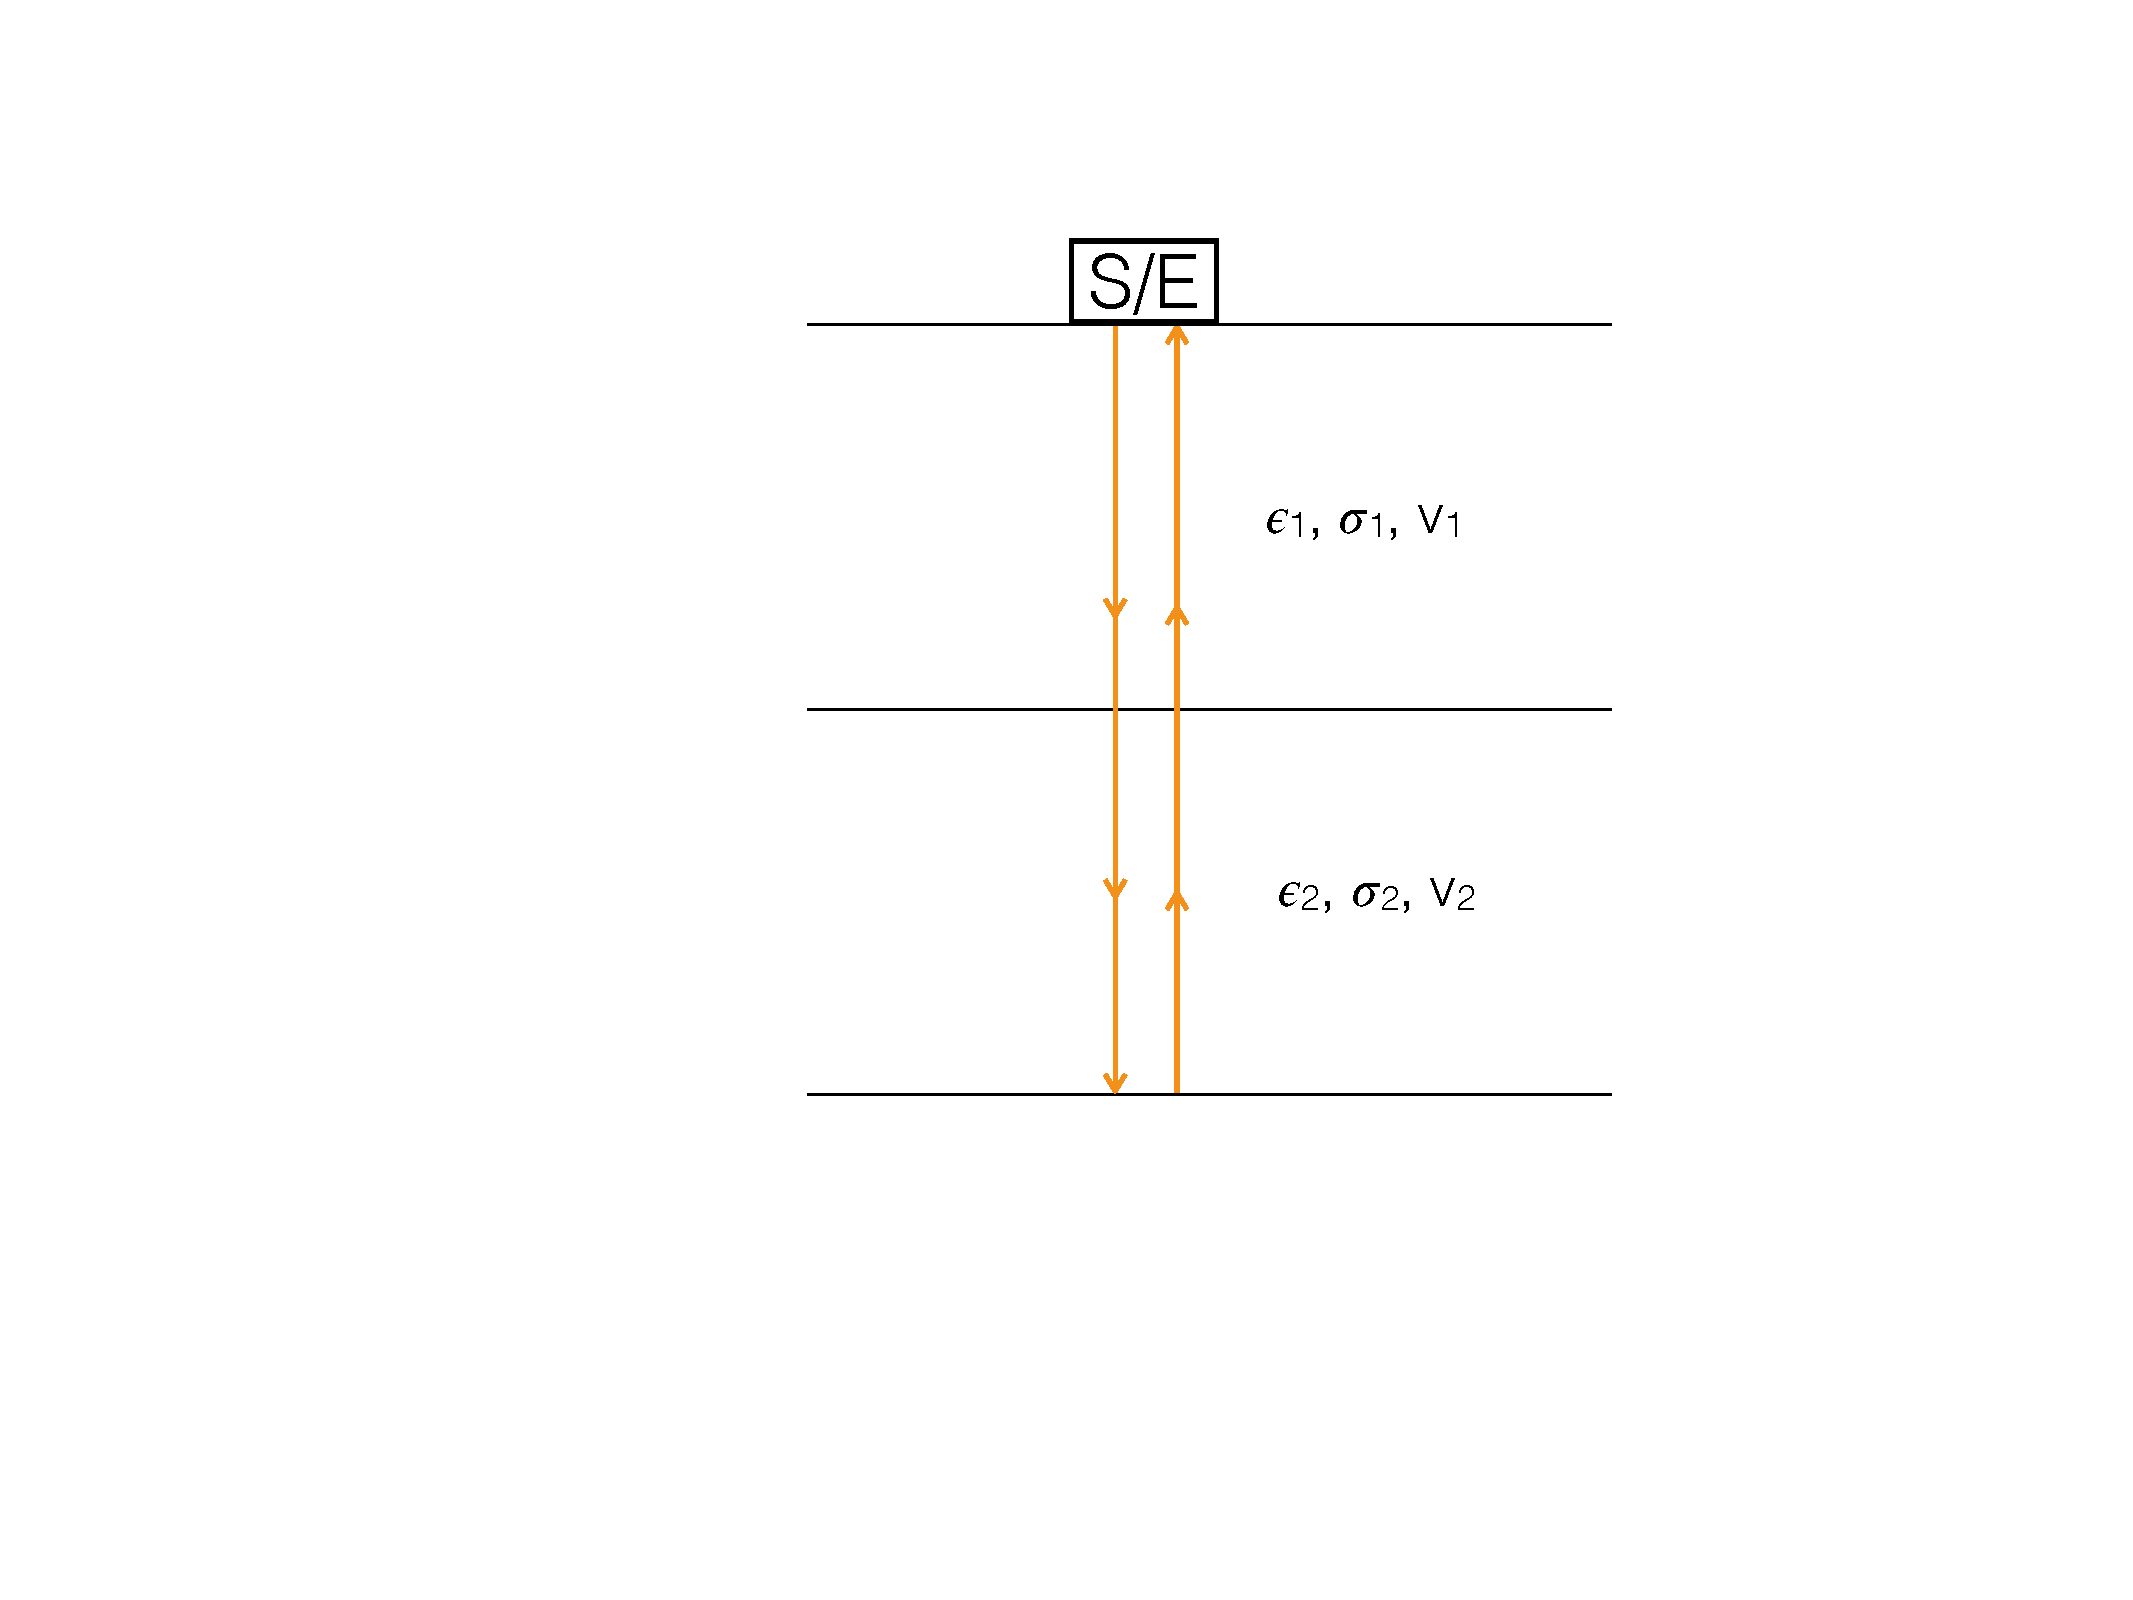
\includegraphics[scale = 0.3]{GeoradarBilder/Monostatisch}
	\caption*{monostatisch}	
	\end{subfigure}
	\begin{subfigure}[m]{0.5\textwidth}
	\centering
		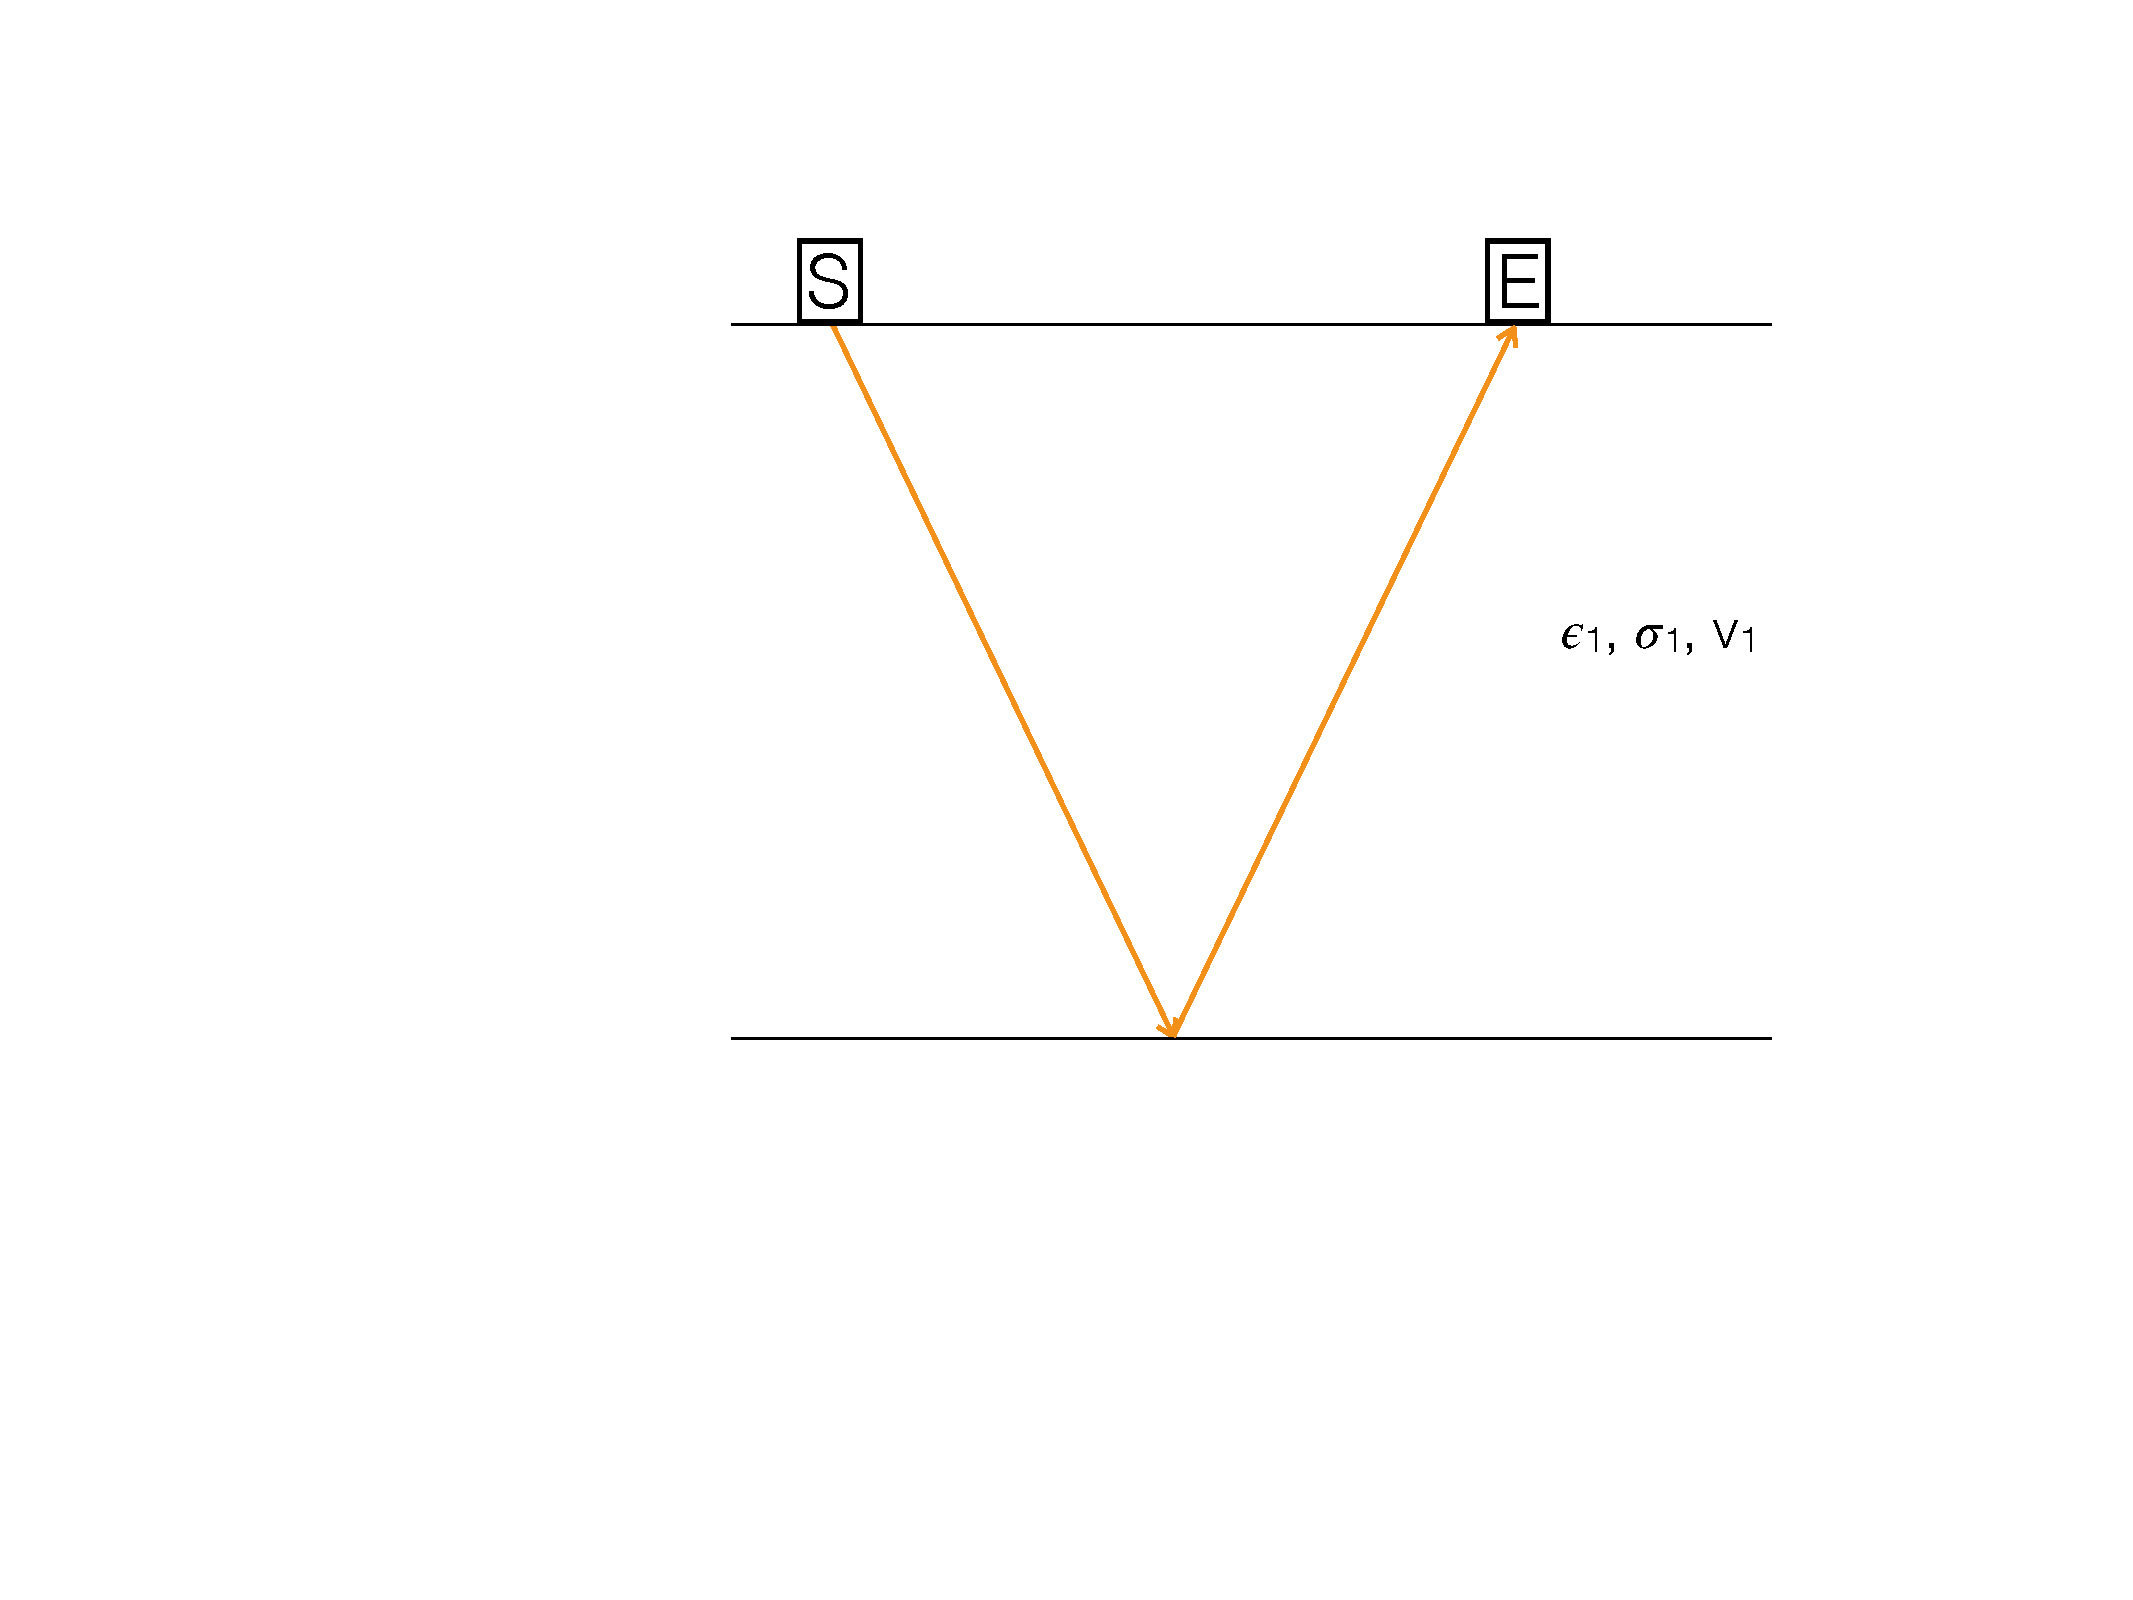
\includegraphics[scale = 0.3]{GeoradarBilder/Bistatisch}
	\caption*{bistatisch}
	\end{subfigure}
\end{figure}


Typisch für eine Messung ist ein bewegter monostatischer Messaufbau. Hierzu wird eine Sender-Empfänger-Kombination entlang einer Messlinie über die Messfläche gezogen. Durch die kontinuierliche Abstrahlung und Registrierung elektromagnetischer Wellen an Sender bzw. Empfänger kann man von einer steten Messung sprechen, d.h. das Messgebiet wird vollständig abgebildet. Die Messdaten werden in ein Radargramm übertragen.

\begin{figure}[H]
	\centering
	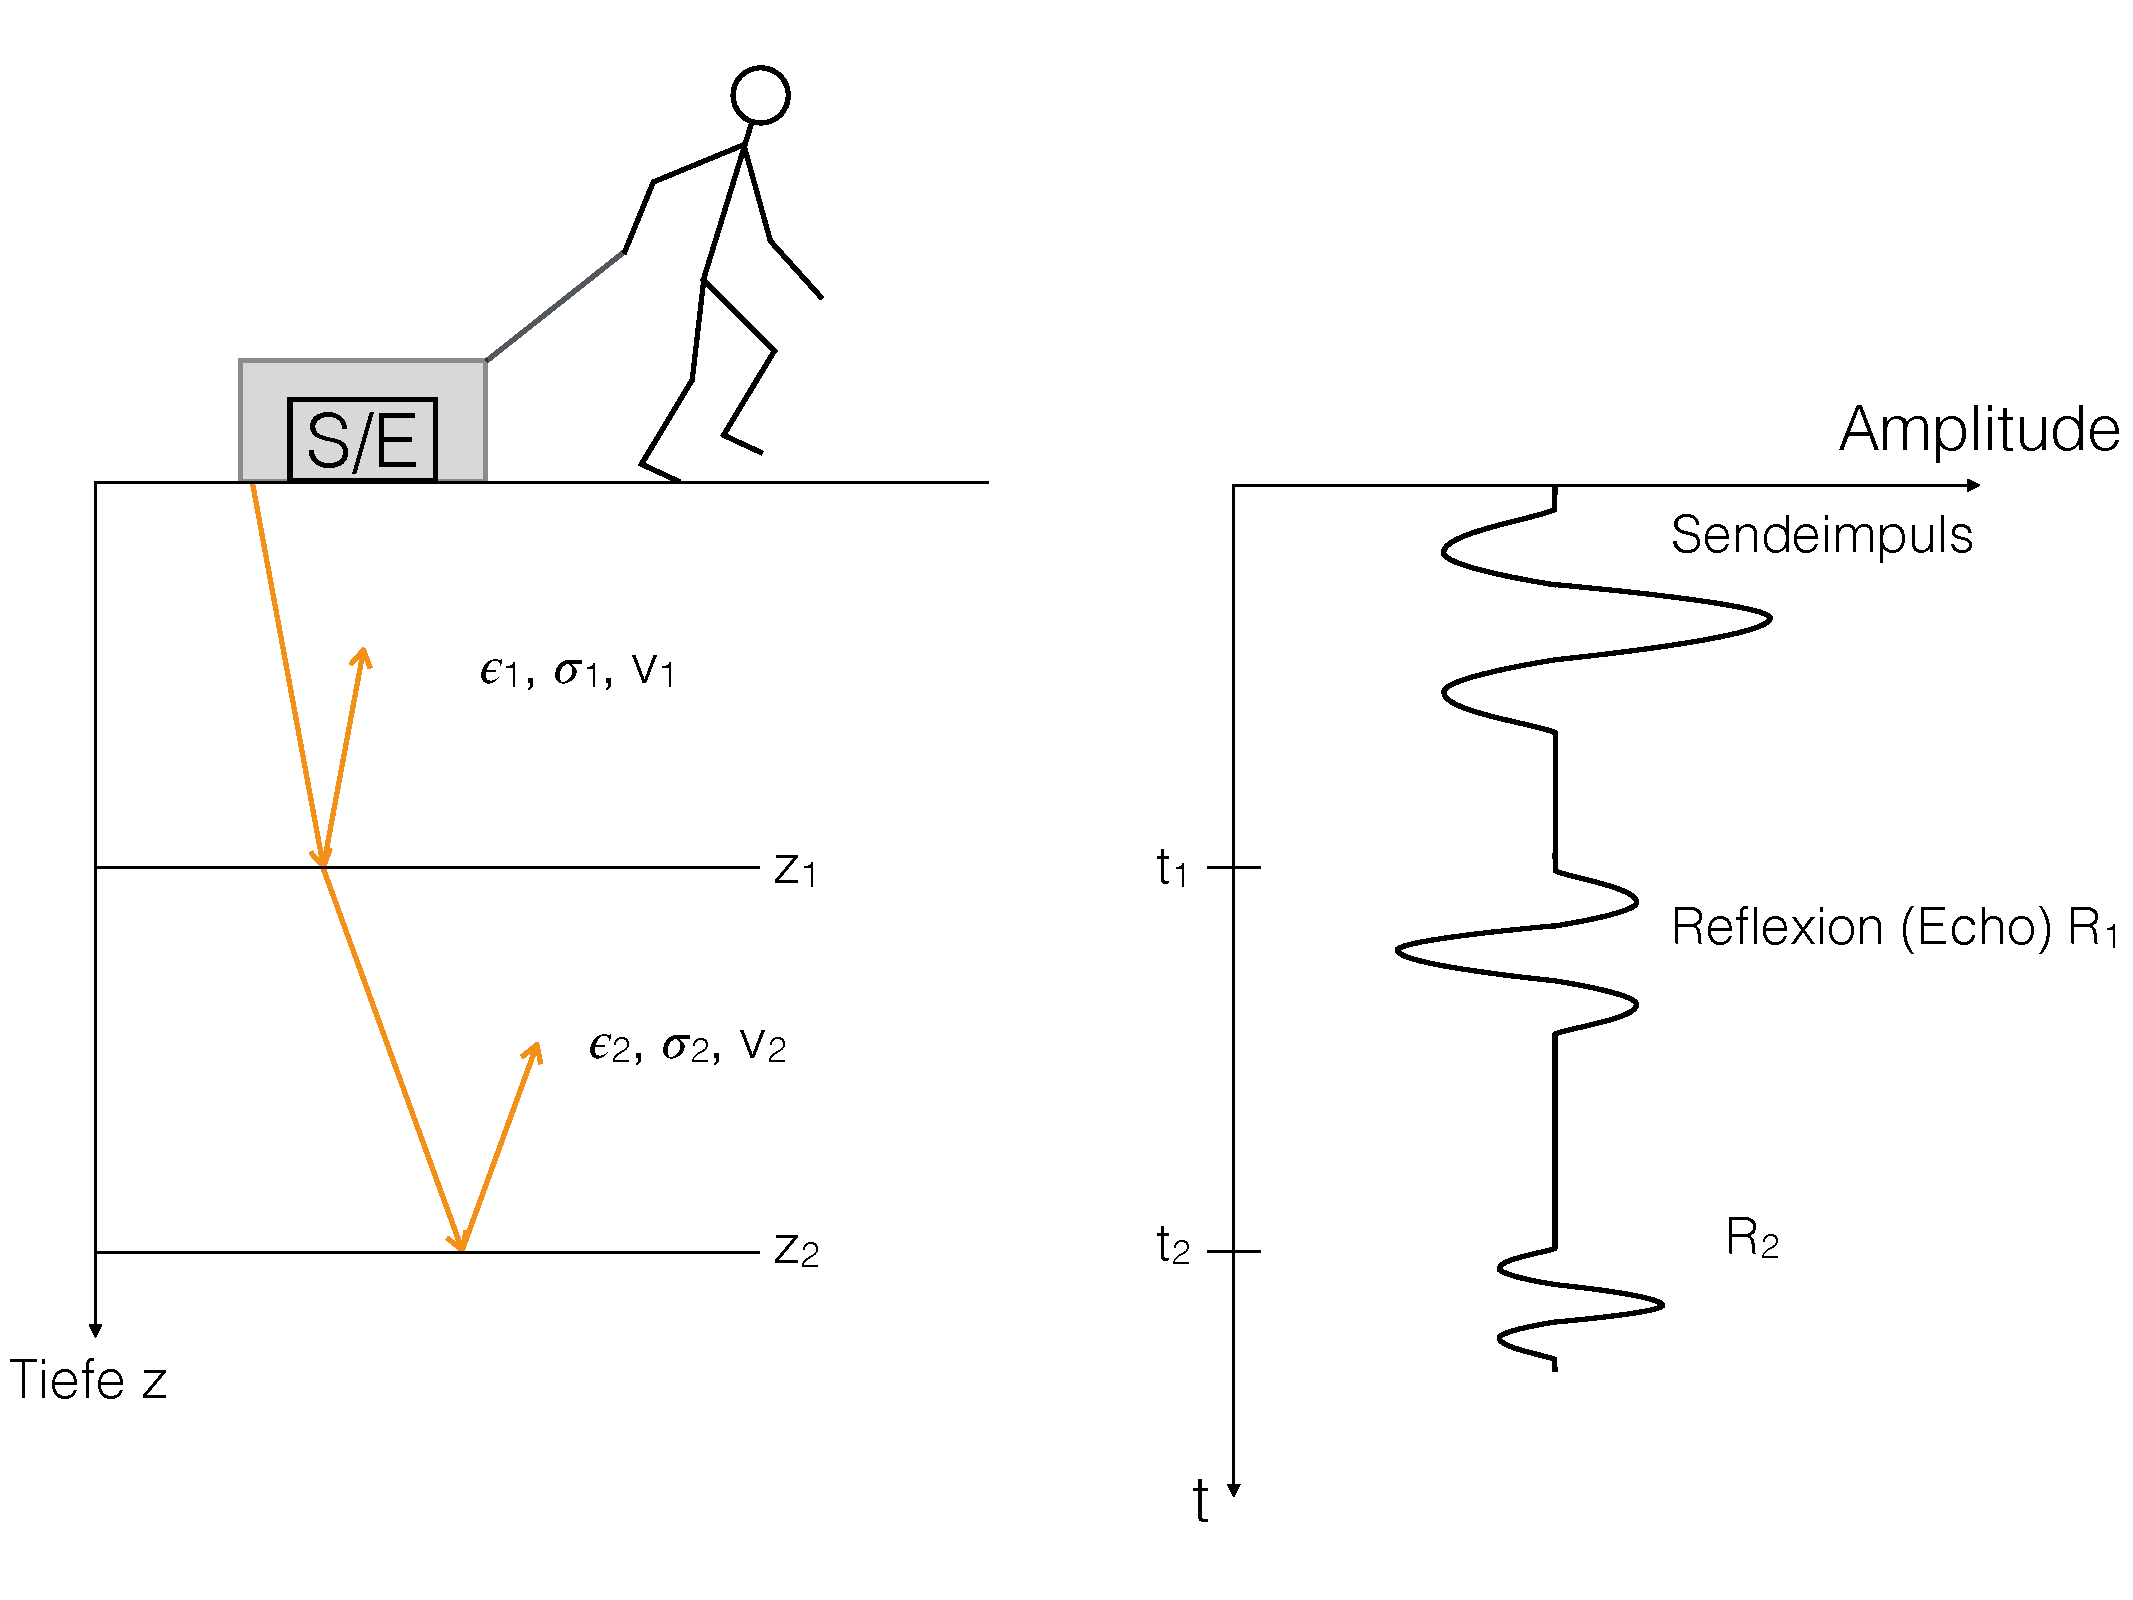
\includegraphics[width = \textwidth]{GeoradarBilder/bewegtMonostatisch}
\end{figure}


\section{Physikalische Parameter}
Die Leitfähigkeit eines Gesteins lässt sich durch zwei physikalische Konstanten beschreiben. Durch Kontrastunterschiede dieser beiden Materialeigenschaften $\epsilon$ und $\sigma$ im Untergrund entstehen Reflexionen und Diffraktionen (Beugungen) der elektromagnetischen Welle.

\subsubsection{Permittivität $\epsilon$} 
Legt man an ein Objekt ein elektrisches Feld an, beginnen sich die freien Ladungsträger des Objektes an diesem Feld auszurichten. Dabei erzeugen sie ein sogenanntes Polarisationsfeld, welches dem äußeren elektrischen Feld entgegenwirkt und dieses abschwächt. Wie stark das Polarisationsfeld wirkt wird mit Hilfe der Materialkonstante $\epsilon_r$ beschrieben. Die Permittivität berechnet sich dann so: \begin{equation*}
	\epsilon = \epsilon_r \cdot \epsilon_0
\end{equation*} Dabei ist $\epsilon_0$ die Permittivität des Vakuums.

\subsubsection*{Elektrische Leitfähigkeit $\sigma$}
Diese Materialgröße gibt an, wie fähig ein Stoff, ist Strom zu leiten.
Grundsätzlich gilt, dass stark wassergesättigte Gesteinsschichten oder tonhaltige Minerale stark leitfähig sind. Aus diesem Grund ist eine Georadarmessung bei solchen Gesteinsschichten nicht möglich.

\section{Auswertung}
Da die Auswertung der Daten aus einer Messung mit Georadar ähnlich der einer reflexionsseismischen Messung sind, möchten wir an dieser Stelle nur auf ein paar Besonderheiten eingehen. 

\subsection{Ausbreitungsgeschwindigkeit}
Wir betrachten zunächst den Normalfall: die Materialeigenschaften des Untergrundes sind bekannt und wir möchten die Geschwindigkeit der elektromagnetischen Wellen berechnen. Hierfür benutzen wir die folgende Formel: \begin{equation*}
	v = \frac{c}{\sqrt{\mu_r \cdot \epsilon_r}} \approx \frac{c}{\sqrt{\epsilon_r}}
\end{equation*}
Hierbei ist $\epsilon_r$ die relative Permittivität, die wir bereits kennengelernt haben. $c$ bezeichnet die Vakuumlichtgeschwindigkeit mit einem Wert von gerundet $3 \cdot 10^{8}\,\si{m/s}$. Die relative Permeabilität wird mit $\mu_r$ angegeben. Dieser Wert ist nur gering variabel und bewegt sich um den Wert 1. Der beeinflussende Faktor für die Wellengeschwindigkeit ist also relative Permittivität. $\epsilon_r$ variiert zwischen Werten von 1 bis 81.

\subsection{Auflösungsvermögen}
Interessant bei einer Messung mit Georadar ist das Auflösungsvermögen der verwendeten Antenne. Dazu muss zunächst der Begriff der \textbf{Nominalfrequenz} geklärt werden. Georadar-Antennen strahlen ihre Energie über eine Bandbreite ab und nicht nur über exakt eine Frequenz. Der Mittelwert dieser Bandbreite ist Nominalfrequenz $f_{\text{N}}$, bei welcher die Antenne also maximal viel Energie abgibt.

Maßgebend für das Auflösungsvermögen ist die räumliche Ausdehnung des elektromagnetischen Pulses (\textbf{Wellenlänge}): \begin{equation*}
	\lambda = \frac{1}{f_{\text{N}}} \cdot v = T \cdot v
\end{equation*} Hierbei ist $v$ die Geschwindigkeit der Radarwelle und T die Pulslänge.

Die theoretische vertikale Auflösung $r$ berechnet sich nun als ein Viertel der Wellenlänge: \begin{equation*}
	r = \frac{1}{4} \lambda
\end{equation*}

\subsection{Auswertung von Diffraktionen}
Trifft die elektromagnetische Welle auf eine kleinräumige Diskontinuität im Untergrund (zum Beispiel eine Rohrleitung, keine Grenzschicht) wird sie wie eine seismische Welle gebrochen und ein Teil wird reflektiert. Diese rückläufige Welle wird an der Oberfläche registriert. Unter der Annahme, dass die Geschwindigkeit $c$ im Medium konstant ist, lässt sich die Tiefe der Diffraktion bestimmen, bzw. umgekehrt die Geschwindigkeit der Welle. Die Formel zur Berechnung wollen wir nun mit Hilfe einer Veranschaulichung des Messaufbaus herleiten.


\begin{figure}[H]
	\centering
	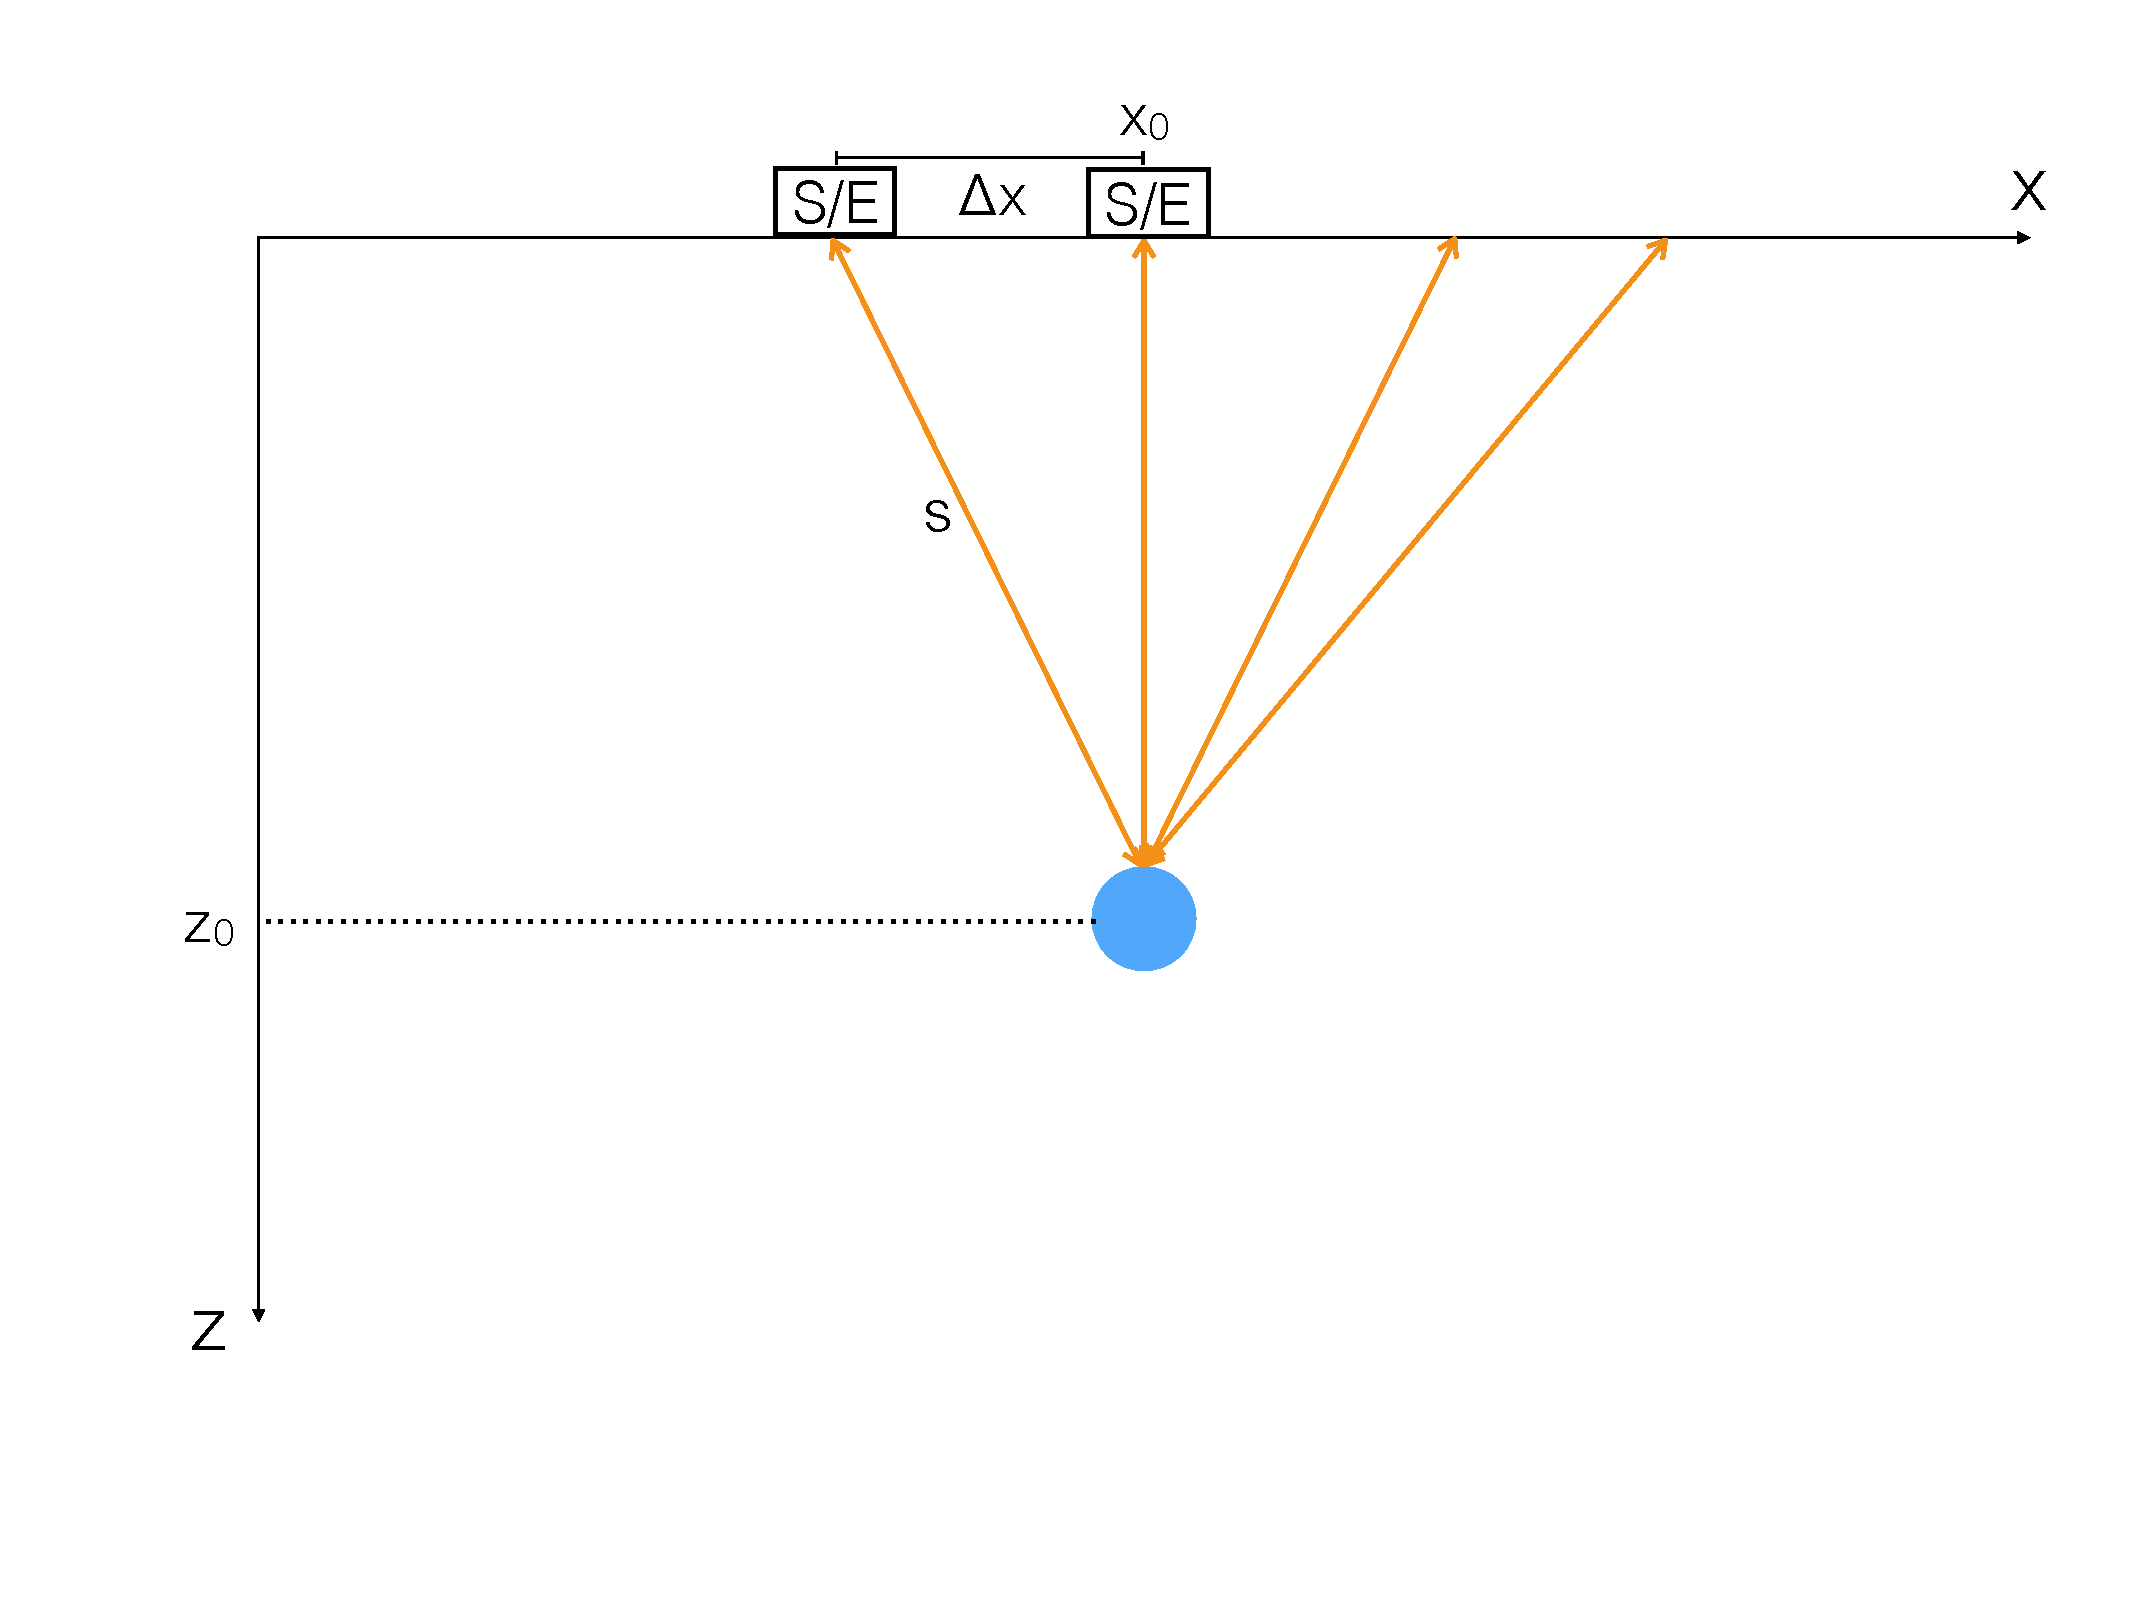
\includegraphics[width = \textwidth]{GeoradarBilder/DiffraktionAufbau}
\end{figure}


Die Laufzeit $t$ berechnet sich so: \begin{equation*}
	t = \frac{2 \cdot s}{v}
\end{equation*}

Diese Gleichung lässt sich unter Kenntnis der Standorte von Sender und Empfänger umformulieren: \begin{equation*}
	t = \frac{2}{v} \cdot \sqrt{\Delta x^2 + z_0^2} = \frac{2}{v} \cdot \sqrt{(x-x_0)^2 + z_0^2}
\end{equation*}

Misst man nun auch noch die Laufzeit $t_0$ der Welle, die im 90$^\circ$-Winkel zur Oberfläche vom Empfänger abstrahlt, lässt sich $z_0$ berechnen: \begin{equation*}
	t_0 = \frac{2 \cdot z_0}{v} \quad \Rightarrow \quad z_0 = \frac{t_0 \cdot v}{2}
\end{equation*}

Daraus ergibt sich nun die Laufzeitgleichung: \begin{equation*}
	t^2 = \frac{4}{v^2} \cdot (\Delta x^2 + z_0^2) = \frac{4}{v^2} \cdot \Delta x^2 + t_0^2
\end{equation*}

Die Gleichung für $t$ ergibt beim Auftragen eine Hyperbel, welche Diffraktionshyperbel genannt wird. 


\begin{figure}[H]
	\centering
	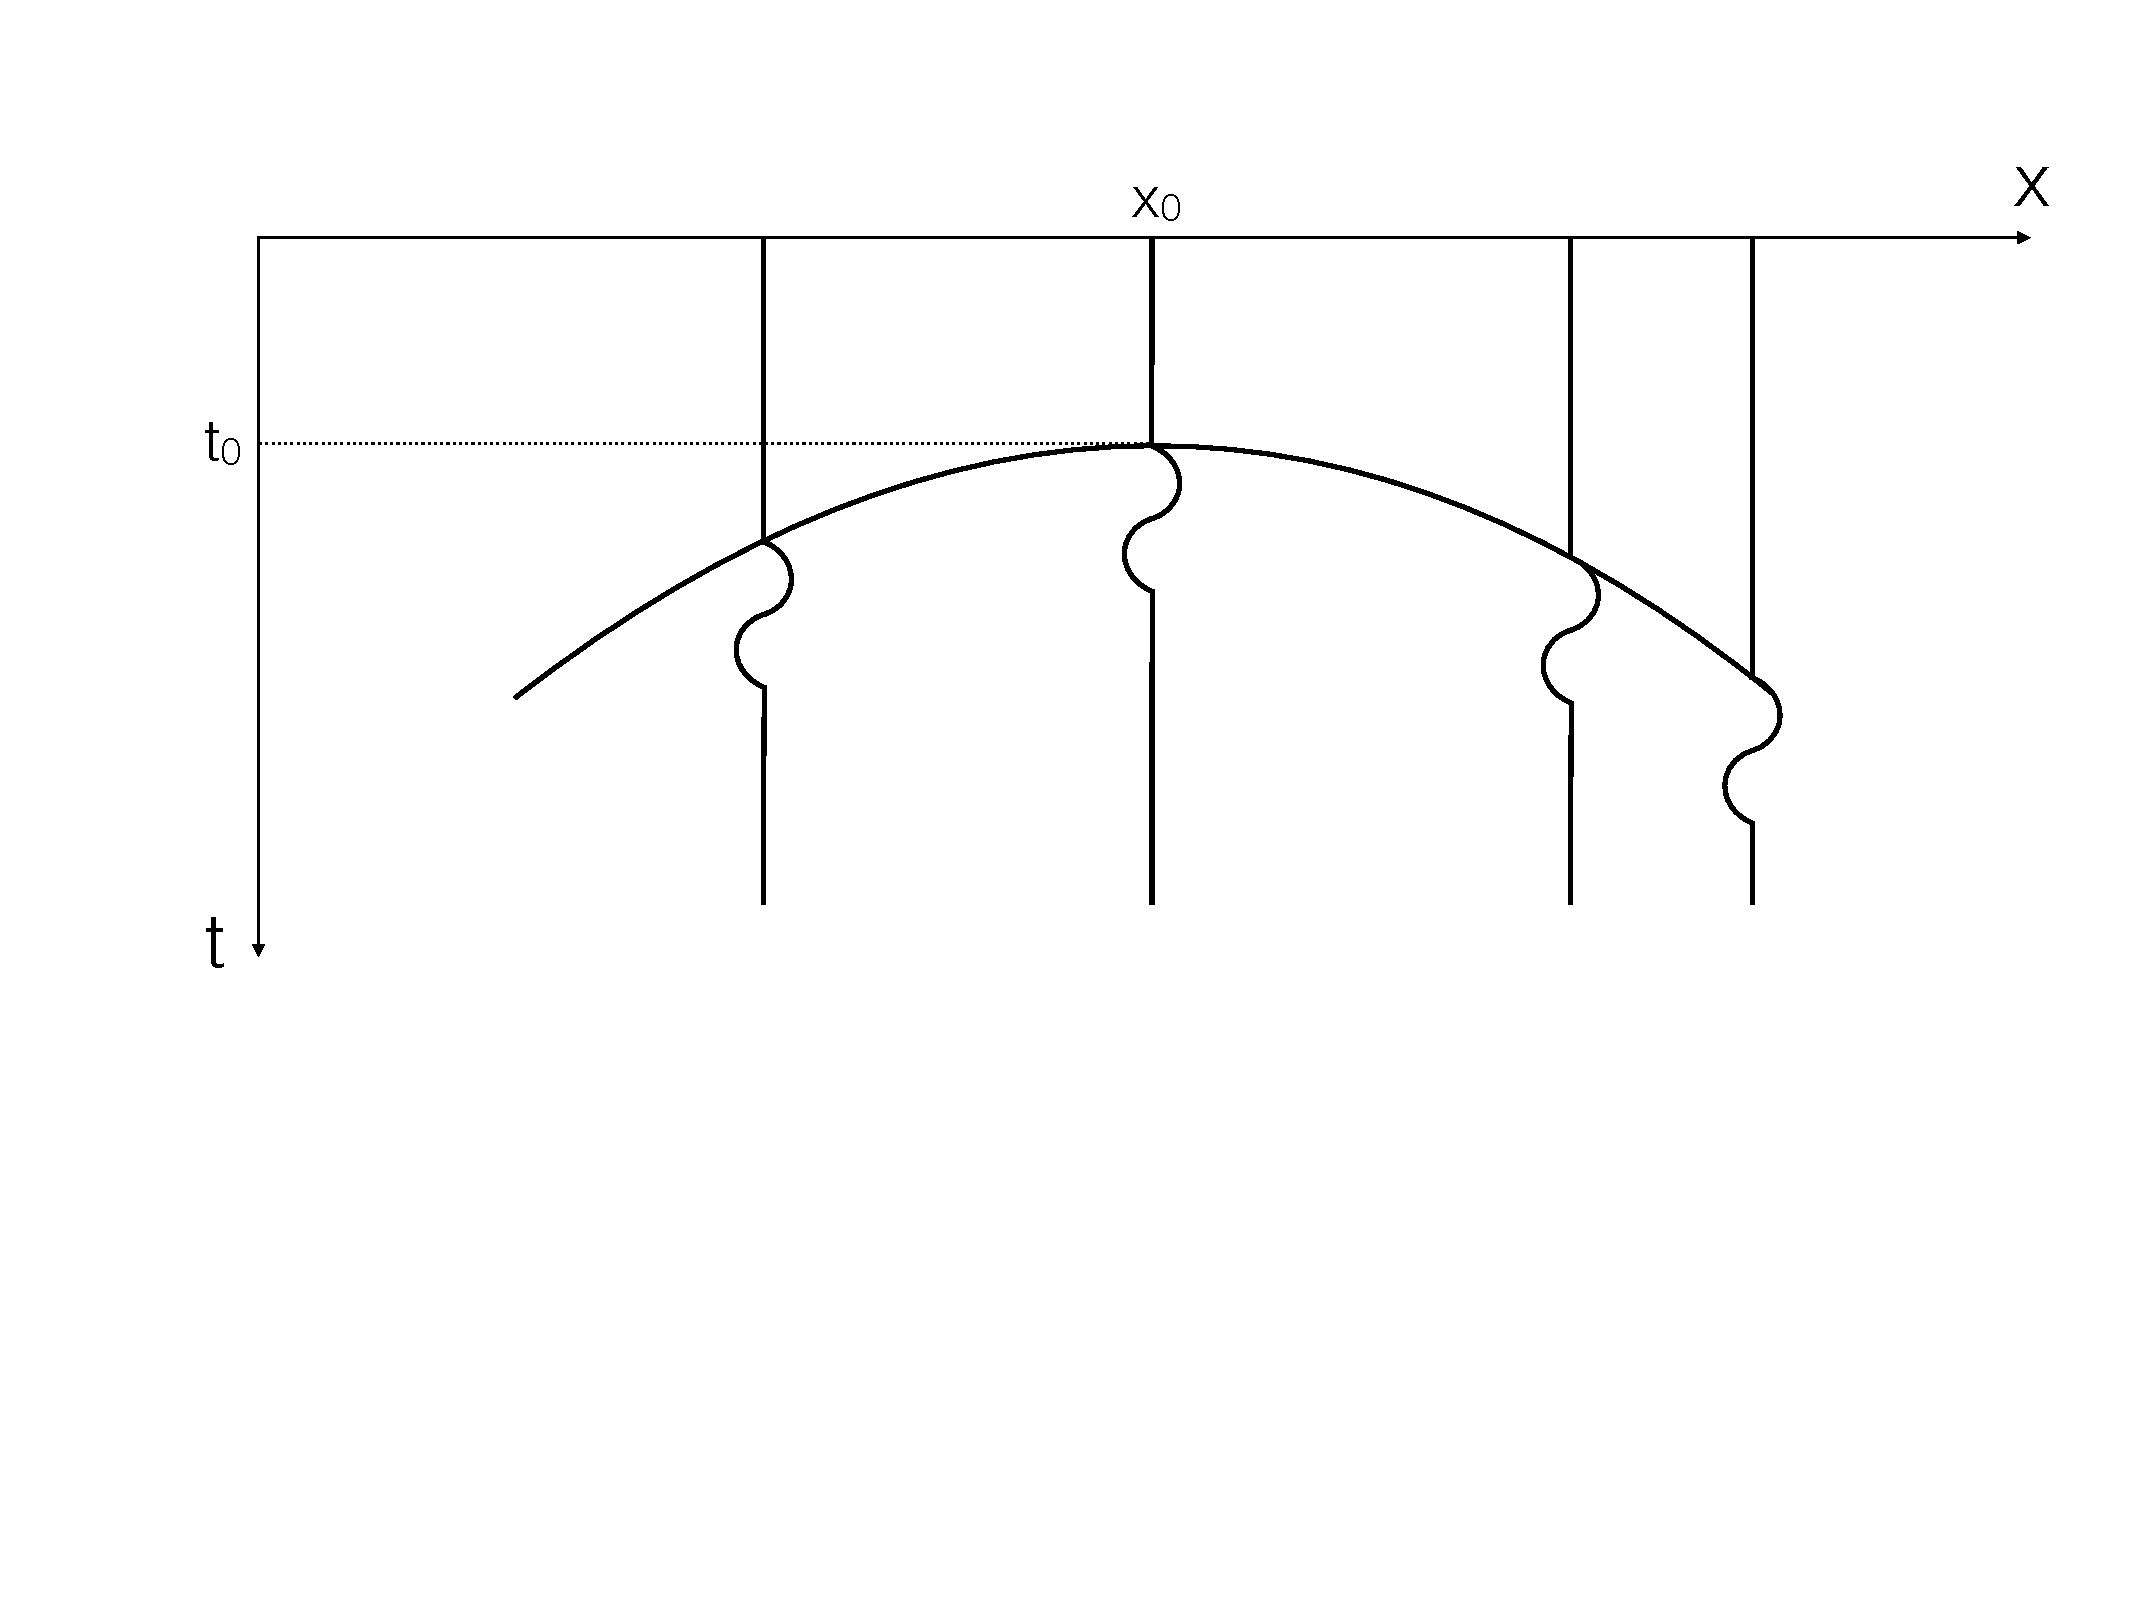
\includegraphics[width = \textwidth]{GeoradarBilder/Radargramm}
\end{figure}

Aus Kenntnis der Geschwindigkeit lassen sich Rückschlüsse über die Materie des Untergrunds ziehen.


\subsection{Reflexionskoeffizient}
Eine weitere Möglichkeit zur Analyse bietet die Reflexionsstärke. Hierbei legt man zu Grunde, dass sich die Permittivität $\epsilon$ an der Grenzschicht signifikant ändert. Der Reflexionskoeffizient lässt sich annähern durch: \begin{equation*}
	R = \frac{\sqrt{\epsilon_2 - \epsilon_1}}{\sqrt{\epsilon_2 + \epsilon_1}}
\end{equation*}

Dies ist die gängige Methode bei Messungen im Feld.














